\documentclass{article}

\usepackage{graphicx}
\usepackage{tikz}
\usepackage{tikzsymbols}
\usetikzlibrary{calc,patterns,shapes.geometric}
\pagestyle{empty}
\usepackage[margin=0pt]{geometry}
\geometry{papersize={14in,12in}}

\def\centerarc[#1](#2)(#3:#4:#5){\draw[#1] ($(#2)+({#5*cos(#3)},{#5*sin(#3)})$) arc (#3:#4:#5);}

\begin{document}
	\begin{figure}
		\centering
		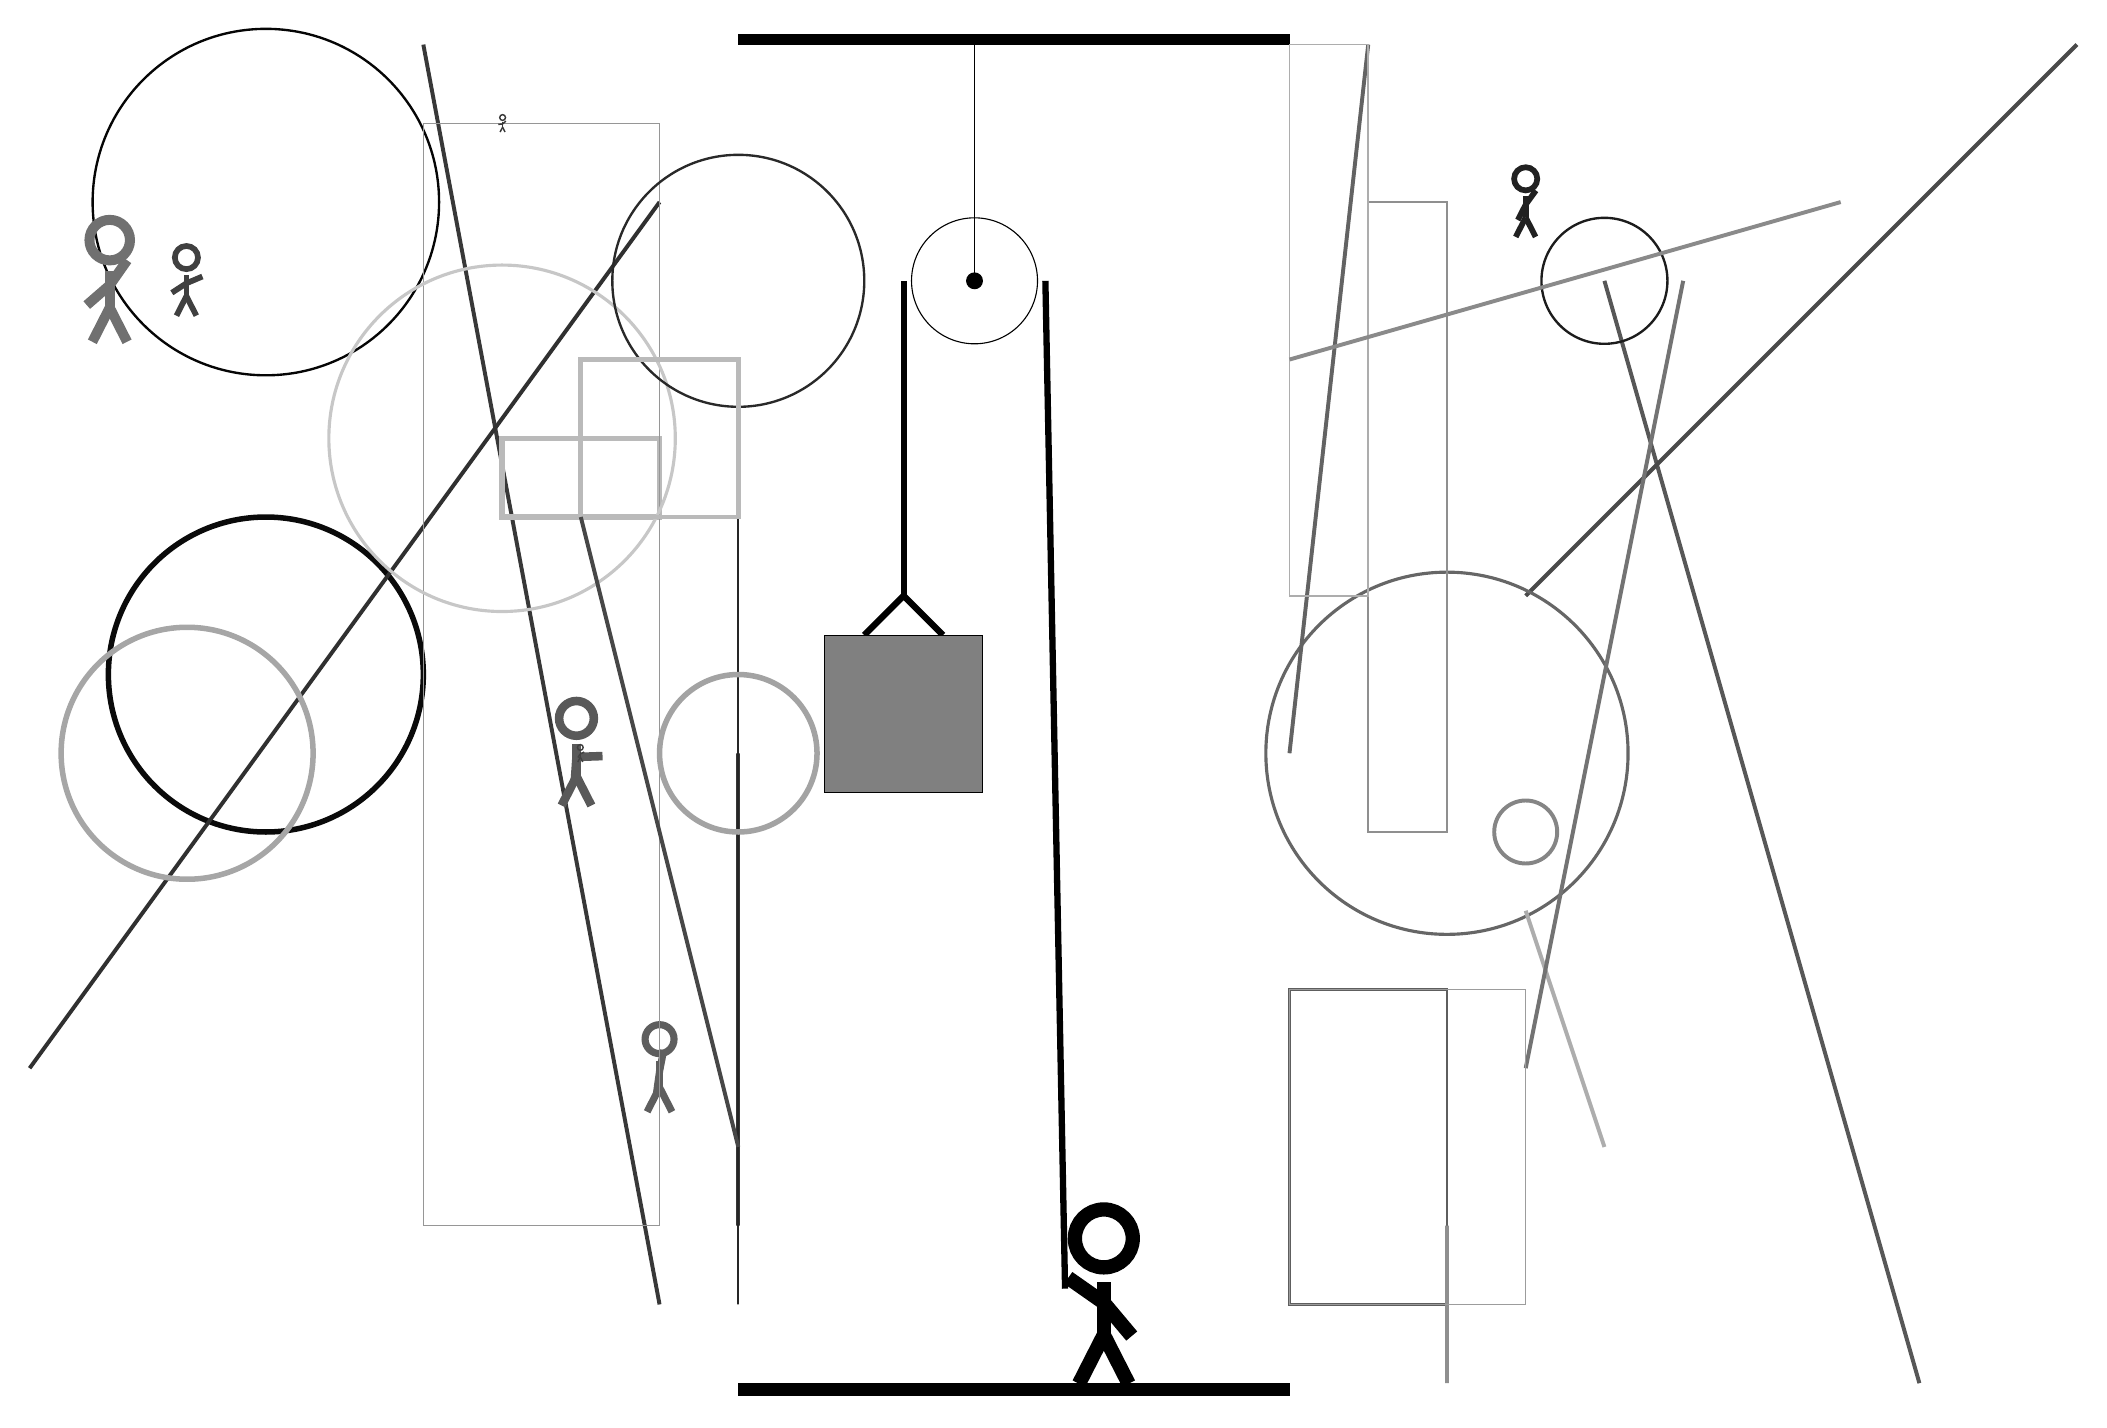
\begin{tikzpicture}
			%%%%% START %%%%%
			
			\draw[fill=black] (-2, 14) rectangle (5, 14.125);
			
			\draw (1, 11) circle (0.8);
			\draw[fill=black] (1, 11) circle (0.1);
			\draw (1, 14) -- (1, 11);
			
			\draw[line width=0.8mm] (-0.4, 6.5) -- (0.1, 7.0) -- (0.6, 6.5);
			\draw[fill=black!50] (-0.9, 6.5) rectangle (1.1, 4.5);
			
			\draw[line width=0.8mm] (0.1, 11) -- (0.1, 7.0);
			\centerarc[line width=0.8mm](1, 11)(0:180:0.9);
			\draw[line width=0.8mm](1.9, 11) -- (2.15, -1.8);
			
			\node at (2.6, -1.9) {\Strichmaxerl[10][-35][-50]};
			
			\draw[line width=0.5mm, color=black!66](9, 11) -- (13, -3);
			
			\node[line width=0.5mm, color=black!63] at (-3, 1) {\Strichmaxerl[5][82][79]};
			\draw [line width=0.3mm, color=black!98](-8, 12) circle (2.2);
			\draw[line width=0.5mm, color=black!78](-6, 14) -- (-3, -2);
			
			\node[line width=0.6mm, color=black!65] at (-4, 5) {\Strichmaxerl[6][86][2]};
			\draw [line width=0.3mm, color=black!89](9, 11) circle (0.8);
			\draw [line width=0.7mm, color=black!96](-8, 6) circle (2.0);
			\draw[line width=0.5mm, color=black!71](8, 7) -- (15, 14);
			\draw [line width=0.7mm, color=black!45](6, 7) circle (0.0);
			
			\draw[line width=0.5mm, color=black!81](-3, 12) -- (-11, 1);
			\node[line width=0.2mm, color=black!56] at (-10, 11) {\Strichmaxerl[7][41][55]};
			
			\draw [line width=0.4mm, color=black!60](7, 5) circle (2.3);
			\draw[line width=0.3mm, color=black!63] (5, 2) rectangle (7, -2);
			\draw[line width=0.5mm, color=black!17] (-2, 3) rectangle (-2, 4);
			\draw[line width=0.7mm, color=black!27] (-3, 9) rectangle (-5, 8);
			\draw[line width=0.2mm, color=black!41] (-3, 13) rectangle (-6, -1);
			
			\draw[line width=0.2mm, color=black!44] (7, 4) rectangle (6, 12);
			\node[line width=0.5mm, color=black!78] at (-5, 13) {\Strichmaxerl[1][6][41]};
			\draw[line width=0.5mm, color=black!32](8, 3) -- (9, 0);
			\draw[line width=0.5mm, color=black!61](6, 14) -- (5, 5);
			\node[line width=0.3mm, color=black!75] at (-9, 11) {\Strichmaxerl[4][33][23]};
			
			\draw [line width=0.4mm, color=black!22](-5, 9) circle (2.2);
			\draw[line width=0.5mm, color=black!55](8, 1) -- (10, 11);
			\draw[line width=0.5mm, color=black!79] (-2, -1) rectangle (-2, 5);
			\draw[line width=0.3mm, color=black!85] (-2, -2) rectangle (-2, 9);
			
			\draw [line width=0.7mm, color=black!35](-9, 5) circle (1.6);
			
			\draw [line width=0.7mm, color=black!36](-2, 5) circle (1.0);
			\draw[line width=0.2mm, color=black!32] (5, 7) rectangle (6, 14);
			
			\draw[line width=0.6mm, color=black!44] (7, -1) rectangle (7, -3);
			\draw[line width=0.5mm, color=black!46](5, 10) -- (12, 12);
			\draw [line width=0.4mm, color=black!79](-7, -2) circle (0.0);
			
			\node[line width=0.6mm, color=black!75] at (-4, 5) {\Strichmaxerl[1][57][25]};
			\draw [line width=0.5mm, color=black!48](8, 4) circle (0.4);
			\draw [line width=0.3mm, color=black!84](-2, 11) circle (1.6);
			\node[line width=0.7mm, color=black!87] at (8, 12) {\Strichmaxerl[4][63][54]};
			\draw[line width=0.2mm, color=black!39] (5, -2) rectangle (8, 2);
			\draw[line width=0.6mm, color=black!27] (-4, 10) rectangle (-2, 8);
			
			\draw[line width=0.5mm, color=black!72](-2, 0) -- (-4, 8);
			
			\draw[fill=black] (-2, -3) rectangle (5, -3.15);
			
			%%%%% END %%%%%
		\end{tikzpicture}
	\end{figure}	
\end{document}